
\documentclass[12pt]{article}
\usepackage{graphicx}


\begin{document}
\begin{titlepage}
\begin{center}

% Upper part of the page. The '~' is needed because \\
% only works if a paragraph has started.


\textsc{ Queensland University of Technology}\\[0.5cm]

\textsc{\Large INN344 Search Engine Technology}\\[3.5cm]

% Title

{ \huge \bfseries Statistical Machine Translator \\[0.4cm] }

% Author and supervisor
\begin{minipage}{0.4\textwidth}
\begin{flushleft} \large
Jussi \textsc{Kolehmainen}
\end{flushleft}
\end{minipage}
\begin{minipage}{0.4\textwidth}
\begin{flushright} \large
n8791023
\end{flushright}

\end{minipage}

\vfill

% Bottom of the page
{\large \today}

\end{center}
\end{titlepage}

\newpage

\section{Introduction}
This document describes one way to implement a statistical machine translation application to the end user.
The approach described here starts with a word-to-word dictionary to translate a sentence word by word.
However, a dictionary may give more than 15 alternatives for a single word.
The main focus of this document is to develop a statistical model, which, together with a large parallel corpus, aims to choose the best translations among the possibilities.

The model developed is somewhat simplified version of some models mentioned in literature.
The simplifications allow faster calculations that, in turn, give shorter response times to the user that is translating a sentence.
At the center of the application is an index that contains all the statistical details needed to rank the translation alternatives in the order of their 


This document begins by describing various machine translation methods before focusing on statistical approaches.
Then, a simplified version for the use of this application is described.
Implementation section defines the technology components that are needed to build a working statistical machine translation application.
Experimental section defines 
At the end we summarize the work and propose future work.



\section{Machine Translation}
\subsection{Approaches}
Machine translation methods can be divided into following categories:
\begin{enumerate}
	\item Dictionary based methods
	\item Rule based methods
	\item Knowledge based methods
	\item Corpus based methods
\end{enumerate}

The model used in this application is a combination of both dictionary and corpus based methods.
The corpus based methods can also be called statistical methods because they employ the statistical features of a large corpus.

More about different methods...




\subsection{General Statistical Model}
Let's assume that we are translating a sentence from Spanish to English. 
We can define a sentence in English by $\mathbf e = (e_1, e_2, ..., e_n)$, where $e_i$ are the single words that construct the sentence.
Similarly, a sentence in Spanish can be defined as $\mathbf{s} = (s_1, s_2, ..., s_n)$.
Our task is to find \textbf{e} that maximizes the conditional probability $P(\mathbf{e}|\mathbf{s})$.
This means that given a sentence \textbf{s} in Spanish, what is the probability that the correct translation in the sentence \textbf{e} in English.

By using the Bayes rule we can write the probability as
\begin{equation}
P(\mathbf{e}|\mathbf{s}) = \frac{P(\mathbf{s}|\mathbf{e}) P(\mathbf{e})}{P(\mathbf{s})}.
\end{equation}
When maximized, the denominator of the previous equation can be neglected because it does not depend on the translation \textbf{e}.
The first part of the equation, $P(\mathbf{s}|\mathbf{e})$, is called translation model.
It is the probability that given a translation \textbf{e}, the initial sentence was \textbf{s}.
The second part of the equation, $P(\mathbf{e})$, is called language model.
It is the probability that the sentence \textbf{e} in the target language is grammatically correct.

The point of using the two models instead of the original probability $P(\mathbf{e}|\mathbf{s})$ is that the inclusion of the language model produces better-formed sentences in the target language. 
Now the problem is to estimate both models from a large parallel corpus, that is, a large number of equivalent sentences in both languages.

The language model probability can be calculated with
\begin{equation}
P(\mathbf{e}) = \prod_{i=1}^m P(e_j | e_1, ..., e_{j-1}),
\end{equation}
where \emph{m} is the number of words in the sentence. 
$P(e_j | e_1, ..., e_{j-1})$ is the probability that, given the beginning of the sentence $(e_1, ..., e_{j-1})$, the next word is $e_j$.
If we take into account only the previous word we simplify calculations significantly.
These probabilities are called bigram probabilities and are calculated as follows
\begin{equation}
P(\mathbf{e}) = P(e_j | e_{j-1}).
\end{equation}

The language model probability for two words $e_1$ and $e_2$ can be estimated from the corpus in the following way:
\begin{equation}
P(e_2 | e_1) = \frac{\#(e_1, e_2)}{\#(e_1)},
\end{equation}
where $\#(e_1, e_2)$ is the number of bigrams with $e_1$ and $e_2$ in the corpus and $\#(e_1)$ is the number of occurences of $e_1$ in the corpus.

This approach, however, fails to estimate probabilities for bigrams that do not occur in the corpus.
By using a linear interpolation between monogram and bigram models we can smooth the model.
\begin{equation}
P(e_2 | e_1) = \lambda \frac{\#(e_2)}{N} + (1 - \lambda) \frac{\#(e_1, e_2)}{\#(e_1)},
\end{equation}
where \emph{N} is the size of the corpus and $\lambda \in \left [ 0,1 \right ]$ is a parameter.
The parameter $\lambda$ should be chosen so that the average probability of the bigrams is maximized when using a second corpus in the same language.

The translation model probability $P(\mathbf{s}|\mathbf{e})$ is much harder to estimate.
It uses the parallel corpus to derive probability distributions that are then used for translating new sentences.
It can be divided into three components:
\begin{enumerate}
	\item Fertility probability $P(n|e)$
	\item Distortion probability $P(i|j,l)$
	\item Translation probability $P(e|s)$
\end{enumerate}

The fertility probability is the probability that the translated word $e$ in English replaces $n$ French words.
The distortion probability is the probability that a Spanish word at the position $i$ in the sentence is replaced with an English word of the length $l$ at the position $j$.
The translation probability is the probability that the Spanish word $s$ is replaced with the English word $e$.

TODO: Estimating the probability distributions

\subsection{Simplified Statistical Model}




\section{Implementation}

\begin{center}
\begin{figure}[h!]
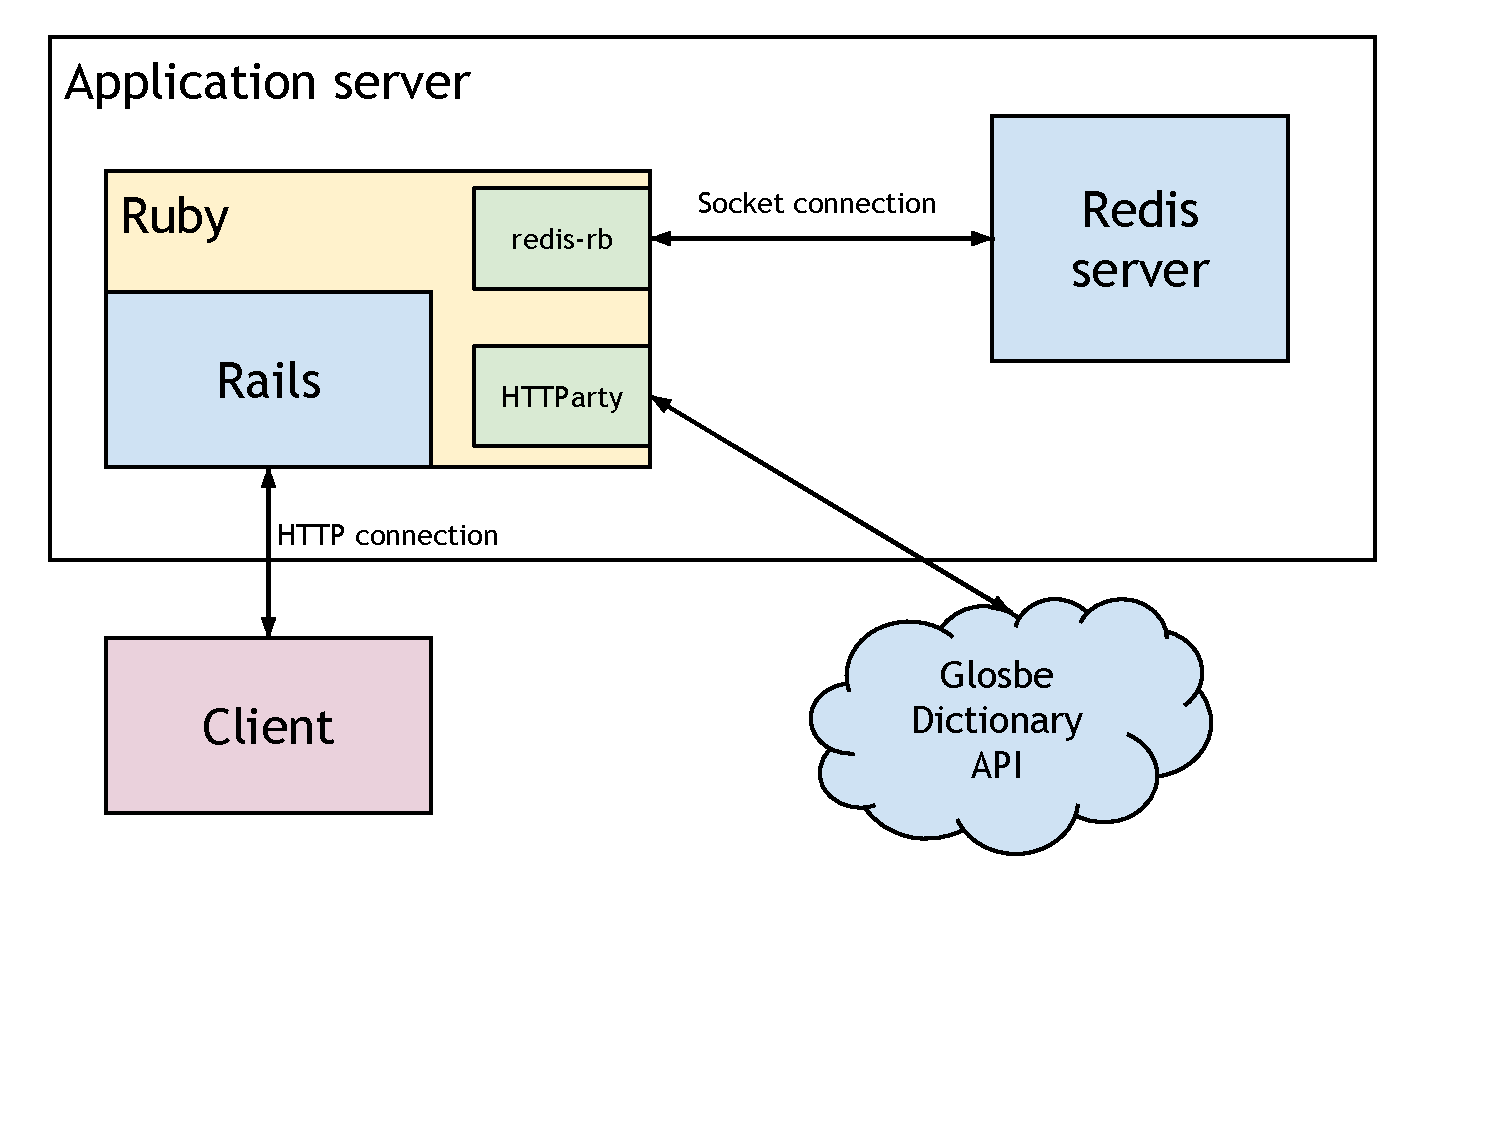
\includegraphics[scale=0.7]{images/arc.pdf}
\caption{System architecture.}
\label{fig:arc}
\end{figure}
\end{center}

The system's architecture is shown in Figure 1.
The application is a Ruby on Rails application and uses several Ruby gems (add-ons).


The application flow goes as follows:
\begin{enumerate}
	\item User types in a sentence to be translated
	\item Client sends the query to the server
	\item Server uses Glosbe Dictionary API to translate words and phrases
	\item Server retrieves corpus statistics from the Redis database
	\item Server calculates probabilities for different translation alternatives
	\item Server returns the translations and their probabilities as JSON
	\item Client shows results to the user
\end{enumerate}


Glosbe Dictionary API responds to HTTP requests of the following form:
\begin{verbatim}
http://glosbe.com/gapi/translate
	?from=[language1]
	&dest=[language2]
	&format=json
	&phrase=[word or phrase]
\end{verbatim}


The index is stored at a Redis server, which is a NoSQL database.
NoSQL database does not have any specific schema but all the data is stored as key-value-pairs.
In this application the following keys are stored when building the index:
\begin{itemize}
	\item term:[lang]:[term] $\rightarrow$ index
	\item term:[lang]:[index] $\rightarrow$ term
	\item term:[lang]:[index]:frequency $\rightarrow$ frequency
	\item term:[lang]:[index]:sentences $\rightarrow$ list of sentence indices
	\item sentence:[lang]:[index] $\rightarrow$ list of word indices
	\item bigram:[lang]:[index1]:[index2] $\rightarrow$ frequency
\end{itemize}

Redis database allows more than 4000 write/read operations per second.
When the index is created, both corpuses are read and the mentioned keys are stored into the database.
When the user submits a sentence to be translated, all the statistics needed for the translation are found from the database.


\section{Experiments}

\subsection{Experimental Design}
Use 90\% of the corpus to estimate the probability distributions and 10\% to evaluate the translator performance.


\subsection{Results}



\section{Conclusions}

\bibliographystyle{abbrv}
\bibliography{main}

\end{document}